The goal of our work is to find bugs in distributed systems \emph{before} they reach production. Typical distributed systems consist of multiple components that interact with each other via \emph{message passing}. If messages---or unexpected failures and timeouts---are not handled properly, they can lead to subtle bugs. To expose these bugs, we use \psharp~\cite{deligiannis2015psharp}, an extension of the \csharp language that provides: (i) language support for \emph{specifying} properties of \emph{correctness}, and \emph{modeling} the environment of distributed systems written in .NET; and (ii) a \emph{systematic testing engine} that can explore interleavings between \emph{distributed events}, such as the nondeterministic order of message deliveries, client requests, failures and timeouts.

Modeling using \psharp involves three core activities. First, the developer must modify the original system so that messages are not sent through the real network, but are instead dispatched through the \texttt{PSharp.Send(...)} method. Such modification does not need to be invasive, as it can be performed using virtual method dispatch, a \csharp language feature widely used for testing. Second, the developer must write a \psharp \emph{test harness} that drives the system towards interesting behaviors by nondeterministically triggering various events (see \S\ref{sec:overview:model}). The harness is essentially a model of the environment of the system. The purpose of these first two activities is to explicitly declare all sources of nondeterminism in the system using \psharp. Finally, the developer must specify the criteria for correctness of an execution of the system-under-test. Specifications in \psharp can encode either \emph{safety} or \emph{liveness}~\cite{lamport1977proving} properties (see \S\ref{sec:overview:safety} and \S\ref{sec:overview:liveness}).

During testing, the \psharp runtime is aware of all sources of nondeterminism that were declared during modeling, and exploits this knowledge to create a scheduling point each time a nondeterministic choice has to be taken. The \psharp testing engine will serialize (in a single-box) the system, and repeatedly execute it from start to completion, each time exploring a potentially different set of nondeterministic choices, until it either reaches a user-supplied bound (e.g.\ in number of executions or time), or it hits a safety or liveness property violation. This testing process is fully automatic and has no false-positives (assuming an accurate test harness). After a bug is discovered, \psharp generates a trace that represents the buggy schedule, which can then be replayed to reproduce the bug. In contrast to logs typically generated during production, the \psharp trace provides a global order of all communication events, and thus is easier to debug.

Due to the highly asynchronous nature of distributed systems, the number of possible states that these systems can reach is exponentially large. Tools such as \textsc{MoDist}~\cite{yang2009modist} and dBug~\cite{simsa2011dbug} focus on testing unmodified distributed systems, but this can easily lead to state-space explosion when trying to exhaustively explore the entire state-space of a production-scale distributed storage system, such as the Azure Storage vNext. On the other hand, techniques such as TLA+~\cite{lamport1994temporal} have been successfully used in industry to verify specifications of complex distributed systems~\cite{newcombe2015aws}, but they are unable to verify the actual implementation.

\begin{figure*}[t]
\centering
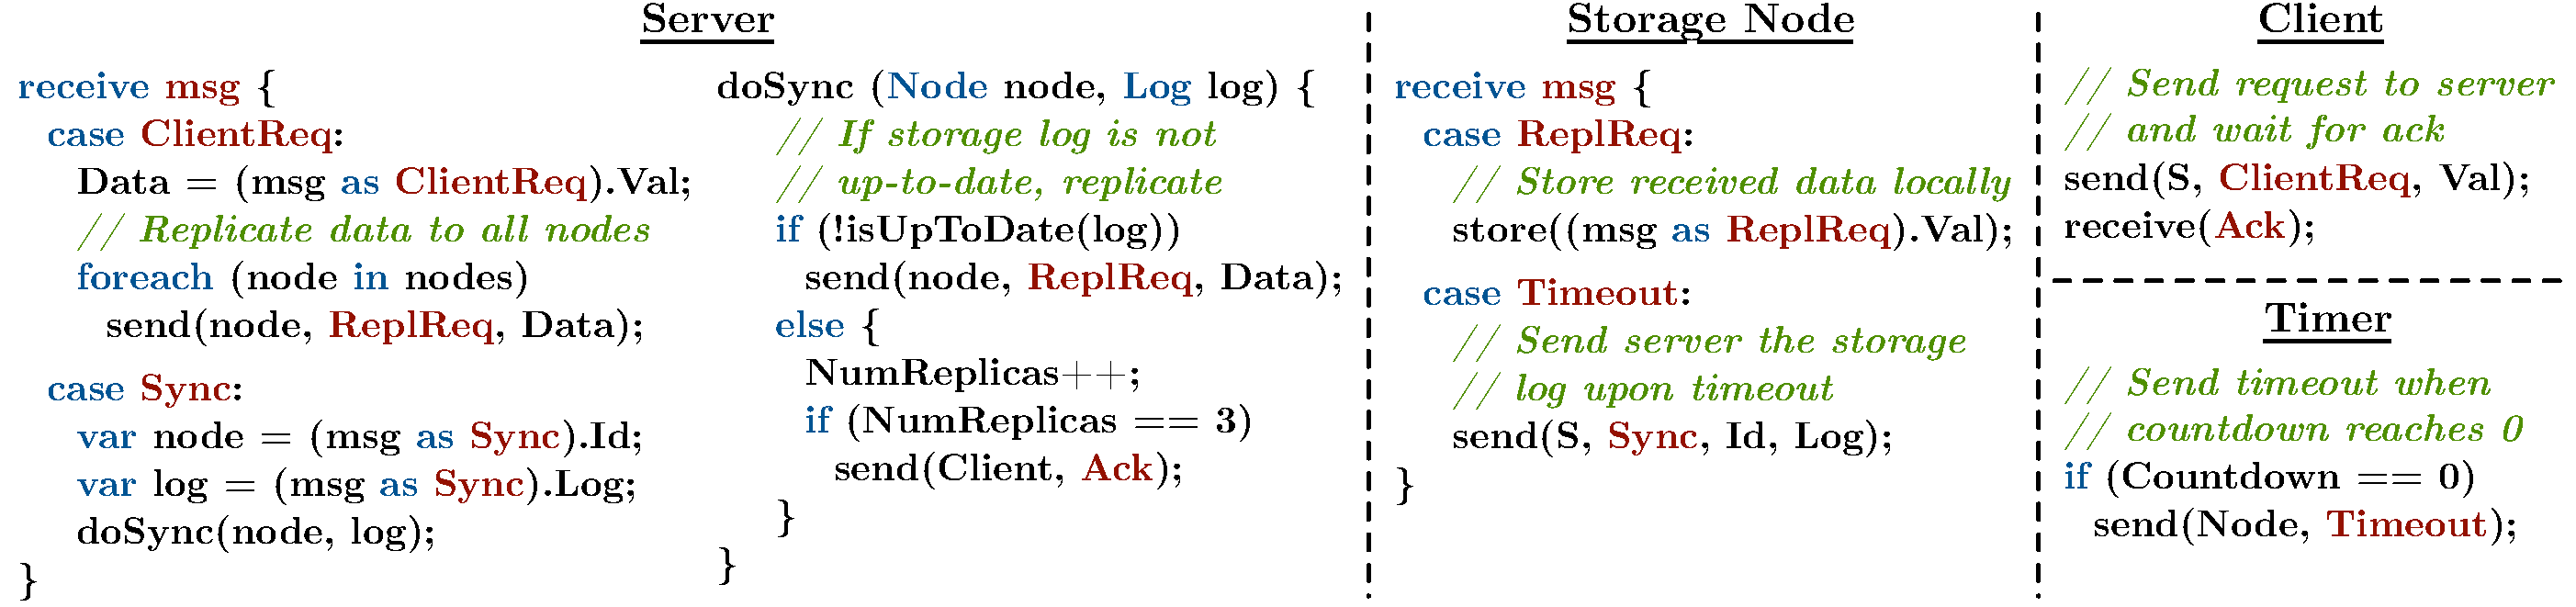
\includegraphics[width=\linewidth]{img/example_code}
\vspace{-7mm}
\caption{Pseudocode of a simple distributed storage system that replicates data sent by a client.}
\label{fig:example}
\vspace{-2mm}
\end{figure*}

In this work, we are proposing a solution between the above two extremes: test the implementation of one or more components against a modeled \psharp environment. The benefit of our approach is that it can detect bugs in the \emph{actual} implementation, but it can do so in a much reduced state-space. Testing with \psharp does not come for free; developers have to invest effort and time into building a test harness using \psharp. However, we argue that developers already spend significant time in building test suites for distributed systems prior to deployment. The \psharp approach augments this effort; by investing time in modeling the environment, it offers dividends by finding more bugs (see \S\ref{sec:eval}). In principle, our methodology is \emph{not specific} to \psharp and the .NET framework, and can be used in combination with any other programming framework that has equivalent capabilities.

\vspace{-2mm}
\subsection{The \psharp programming model}
\label{sec:overview:psharp}

\psharp programs consist of multiple \emph{state machines} that communicate with each other \emph{asynchronously} by exchanging \emph{events}. In the case of distributed systems, \psharp events can be used to model regular messages between system components, failures or timeouts. A \psharp machine declaration is similar to a \csharp class declaration, but a machine also contains an event queue, and one or more \emph{states}. Each state can register \emph{actions} to handle incoming events.

\psharp machines run concurrently with each other, each executing an event handling loop that dequeues the next event from the queue and handles it by invoking the registered action. An action might transition the machine to a new state, create a new machine, send an event to another machine, access a field or call a method. In \psharp, a send operation is \emph{non-blocking}; the event is simply enqueued into the queue of the target machine, which will dequeue and handle the event concurrently. All this functionality is provided in a lightweight runtime library, built on top of Microsoft's Task Parallel Library~\cite{leijen2009tpl}.

\vspace{-2mm}
\subsection{An example distributed system}
\label{sec:overview:example}

Figure~\ref{fig:example} presents the pseudocode of a simple distributed storage system that was contrived for the purposes of explaining our testing methodology. The system consists of a client, a server and three storage nodes (SNs). The client sends the server a \texttt{ClientReq} message that contains data to be replicated, and then waits to get an acknowledgement before sending the next request. When the server receives \texttt{ClientReq}, it first stores the data locally (in the \texttt{Data} field), and then broadcasts a \texttt{ReplReq} message to all SNs. When an SN receives \texttt{ReplReq}, it handles the message by storing the received data locally (using the \texttt{store} method). Each SN has a timer installed, which sends periodic \texttt{Timeout} messages. Upon receiving \texttt{Timeout}, an SN sends a \texttt{Sync} message to the server that contains the storage log. The server handles \texttt{Sync} by calling the \texttt{isUpToDate} method to check if the SN log is up-to-date. If it is not, the server sends a repeat \texttt{ReplReq} message to the outdated SN. If the SN log is up-to-date, then the server increments a replica counter by one. Finally, when there are three replicas available, the server sends an \texttt{Ack} message to the client.

There are two bugs in the above example. The first bug is that the server does not keep track of unique replicas. The replica counter increments upon each up-to-date \texttt{Sync}, even if the syncing SN is already considered a replica. This means that the server might send \texttt{Ack} when fewer than three replicas exist, which is erroneous behaviour. The second bug is that the server does not reset the replica counter to 0 upon sending an \texttt{Ack}. This means that when the client sends another \texttt{ClientReq}, it will never receive \texttt{Ack}, and thus block indefinitely.

\vspace{-1mm}
\subsection{Modeling the example system}
\label{sec:overview:model}

To systematically test the example of Figure~\ref{fig:example}, the developer must first create a \psharp test harness, and then specify the correctness properties of the system. Figure~\ref{fig:example:model} illustrates a test harness that can find the two bugs discussed in \S\ref{sec:overview:example}. Each box in the figure represents a concurrently running \psharp machine, while an arrow represents an event being sent from one machine to another. We use three types of boxes: (i) a box with rounded corners and thick border denotes a real component wrapped inside a \psharp machine; (ii) a box with thin border denotes a modeled component in \psharp; and (iii) a box with dashed border denotes a special \psharp machine used for safety or liveness checking (see \S\ref{sec:overview:safety} and \S\ref{sec:overview:liveness}).

We do not model the server component since we want to test its actual implementation. The server is wrapped inside a \psharp machine, which is responsible for: (i) sending events via the \texttt{PSharp.Send(...)} method, instead of the real network; and (ii) delivering received events to the wrapped component. We model the SNs so that they store data in memory rather than on disk (which could be inefficient during testing). We also model the client so that it can drive the system by repeatedly sending a \texttt{ClientReq} and then waiting for an \texttt{Ack}. Finally, we model the timer so that \psharp takes control of all time-related nondeterminism in the system. This allows the \psharp runtime to control when a \texttt{Timeout} event will be sent to the SNs during testing, and systematically explore different schedules.

\psharp uses object-oriented language features such as interfaces and virtual method dispatch to connect the real code with the modeled code. Programmers in industry are used to working with such features, and heavily employ them in production for testing purposes. In our experience, this significantly lowers the bar for engineering teams inside Microsoft to embrace \psharp for testing.

In \S\ref{sec:overview:safety} and \S\ref{sec:overview:liveness}, we discuss how safety and liveness specifications can be expressed in \psharp to check if the example is correct. The interested reader can refer to the \psharp GitHub repository\footnote{\url{https://github.com/p-org/PSharp}} to find a manual and samples (e.g.\ Paxos~\cite{lamport1998part} and Raft~\cite{ongaro2014raft}), and read \S\ref{sec:vnext}, \S\ref{sec:migrating} and \S\ref{sec:fabric} to learn more details about how \psharp was used to model and test real distributed storage systems in Microsoft.

\vspace{-1mm}
\subsection{Specifying safety properties in \psharp}
\label{sec:overview:safety}

\begin{figure}[t]
\centering
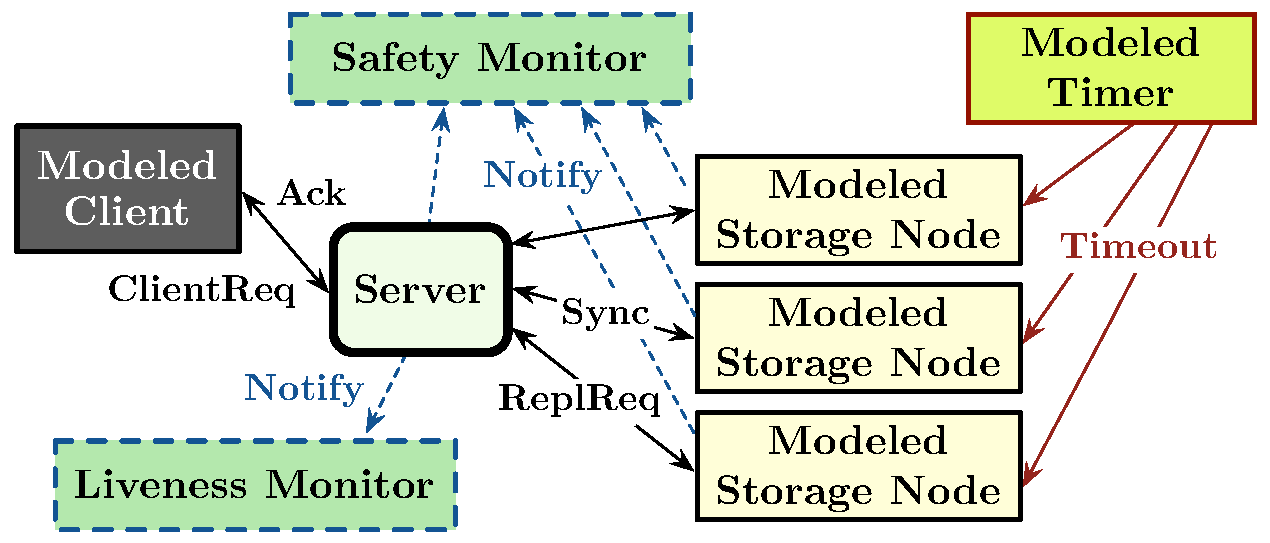
\includegraphics[width=\linewidth]{img/example}
\vspace{-5mm}
\caption{\psharp test harness for the Figure~\ref{fig:example} example.}
\label{fig:example:model}
\vspace{-2mm}
\end{figure}

Safety property specifications generalize the notion of source code assertions; a safety violation is a finite trace leading to an erroneous state. \psharp supports the usual assertions for specifying safety properties that are local to a \psharp machine, and also provides a way to specify global assertions by using a \emph{safety monitor}~\cite{desai2015building}, a special \psharp machine that can receive, but not send, events.

A safety monitor maintains local state that is modified in response to events received from ordinary (non-monitor) machines. This local state is used to maintain a history of the computation that is relevant to the property being specified. An erroneous global behavior is flagged via an assertion on the private state of the safety monitor. Thus, a monitor cleanly separates instrumentation state required for specification (inside the monitor) from program state (outside the monitor).

The first bug in the example of \S\ref{sec:overview:example} is a safety bug. To find it, the developer can write a safety monitor (see Figure~\ref{fig:example:model}) that contains a map from unique SN ids to a Boolean value, which denotes if the SN is a replica or not. Each time an SN replicates the latest data, it notifies the monitor to update the map. Each time the server issues an \texttt{Ack}, it also notifies the monitor. If the monitor detects that an \texttt{Ack} was sent without three replicas actually existing, a safety violation is triggered.

\vspace{-1mm}
\subsection{Specifying liveness properties in \psharp}
\label{sec:overview:liveness}

Liveness property specifications generalize nontermination; a liveness violation is an infinite trace that exhibits lack of progress. Typically, a liveness property is specified via a temporal logic formula~\cite{Pnueli1977, lamport1994temporal}. We take a different approach and allow the programmer to write a \emph{liveness monitor}~\cite{desai2015building}. Similar to a safety monitor, a liveness monitor can receive, but not send, events.

A liveness monitor contains two special types of states: \emph{hot} and \emph{cold}. A hot state denotes a point in the execution where progress is required but has not happened yet; e.g.\ a node has failed but a new one has not come up yet. A liveness monitor enters a hot state when it is notified that the system must make progress. The liveness monitor leaves the hot state and enters a cold state when it is notified that the system has progressed. An infinite execution is erroneous if the liveness monitor is in a hot state for an infinitely long time. Our liveness monitors can encode arbitrary temporal logic properties.
%A thermometer analogy is useful for understanding liveness monitors: a hot state increases the temperature by a small value; a cold state resets the temperature to zero; a liveness error happens if the temperature becomes infinite.
%The distinction between ordinary and cold states is useful for modeling progress for each instance of an infinite stream of events, such as a periodic request or a periodic timer expiration.

A liveness violation is witnessed by an \emph{infinite} execution in which all concurrently executing \psharp machines are \emph{fairly} scheduled. Unfortunately, it is clearly not possible to generate an infinite execution by executing a program for a finite amount of time. Therefore, our implementation of liveness checking in \psharp approximates an infinite execution using several heuristics. In this work, we consider an execution longer than a large user-supplied bound as an ``infinite'' execution~\cite{killian2007life, musuvathi2008fair}. Note that fairness is not relevant when using this heuristic, due to our pragmatic use of a large bound instead of proper handling of infinite executions.

%Another heuristic maintains a cache of (pieces of) the state of the \psharp program obtained at each step in the execution, and reports an ``infinite'' execution when the latest step results in a cache hit, thus approximating a cycle in the state graph of the program.

The second bug in the example of \S\ref{sec:overview:example} is a liveness bug. To detect it, the developer can write a liveness monitor (see Figure~\ref{fig:example:model}) that transitions from a hot state, which denotes that the client sent a \texttt{ClientReq} and waits for an \texttt{Ack}, to a cold state, which denotes that the server has sent an \texttt{Ack} in response to the last \texttt{ClientReq}. Each time a server receives a \texttt{ClientReq}, it notifies the monitor to transition to the hot state. Each time the server issues an \texttt{Ack}, it notifies the monitor to transition to the cold state. If the monitor is in a hot state when the bounded infinite execution terminates, a liveness violation is triggered.

%\textbf{Using monitors}.
%To declare a safety or a liveness monitor, the programmer must inherit from the \psharp \texttt{Monitor} class. \psharp monitors are singleton instances and, thus, an ordinary machine does not need a reference to a monitor to send it an event. Instead, an ordinary machine can invoke a monitor by calling \texttt{Monitor<M>(e, p)}, where the parameter \texttt{e} is the event being send, and the parameter \texttt{p} is an optional payload.

%\subsection{Modeling and testing with \psharp}
%\label{sec:overview:test}

%To detect the two bugs in the example system of Figure~\ref{fig:example}, the developer must first model the system using \psharp and then specify its correctness properties. Figure~\ref{fig:example:model} illustrates a test harness written in \psharp that can be used for finding the bugs in the example system of Figure~\ref{fig:example}.
%
%Our approach of using \psharp to find distributed system bugs requires the developer to perform the following three key modeling tasks. These tasks are illustrated in \S\ref{sec:method} for the Azure Storage vNext system.
%
%\begin{enumerate}
%\item The real components of a distributed system must be wrapped inside \psharp machines. In addition, all the asynchrony due to message passing in the system must be modeled using the \psharp event-sending APIs. 
%
%\item The environment of the system must be modeled in \psharp, which offers APIs for obtaining non-deterministically chosen values. These values can be used to simulate failures, timers, etc. (see \S\ref{sec:method:timer} and \S\ref{sec:method:driver}). This step captures external sources of nondeterminism. The \psharp testing engine can then systematically explore all choices, enumerating different asynchronous event interleavings, possible points of failures, timers firing, etc.
%\end{enumerate}

%\noindent
%We collectively refer to the environment model of a system and its wrapped components as the \psharp \emph{test harness}. This test harness can be used by \psharp to drive the system towards interesting behaviors. \psharp uses modern object-oriented language features such as \emph{interfaces} and \emph{virtual method dispatch} to connect the real code with the modeled code. Programmers in industry are used to working with such features, and heavily use them in production for testing purposes. In our experience, this significantly lowers the bar for engineering teams inside Microsoft to embrace \psharp for testing.

%In principle, our modeling methodology is \emph{not specific} to \psharp and the .NET framework, and can be used in combination with any other programming framework that has equivalent capabilities.
%We also argue that our approach is \emph{flexible} since it allows the user to model \emph{as much} or \emph{as little} of the environment as required to achieve the desired level of testing.

%A key capability of the \psharp runtime is that it can execute in \emph{bug-finding} mode, which systematically tests a \psharp program to find bugs using the safety and liveness monitors that were discussed in \S\ref{sec:overview:specs}.

%When the \psharp runtime executes in bug-finding mode, an embedded \emph{systematic concurrency testing engine}~\cite{godefroid1997verisoft, musuvathi2008finding, emmi2011delay} captures and takes control of all sources of non-determinism that are \emph{known} to the \psharp runtime. In particular, the runtime is aware of nondeterminism due to the interleaving of event handlers in different machines. Each send operation to an ordinary (non-monitor) machine, and each create operation of an ordinary machine, creates an interleaving point where the runtime makes a scheduling decision. The runtime is also aware of all nondeterministic events (e.g. failures) that were captured during the modeling process.

%We have implemented two different schedulers that are responsible for making scheduling and other non-deterministic choices: a \emph{random} scheduler that makes each nondeterministic choice randomly, and a \emph{probabilistic concurrency testing}~\cite{burckhardt2010pct} (PCT) scheduler. It is straightforward to create a new scheduler by implementing the \texttt{ISchedulingStrategy} interface~\cite{desai2015systematic} exposed by the \psharp libraries. The interface exposes callbacks that are invoked by the \psharp testing engine for taking decisions regarding which machine to schedule next, and can be used for developing both generic and application-specific schedulers.

%\textbf{Handling \csharp 5.0 asynchrony}.
%Our case studies heavily use the \texttt{async} and \texttt{await} \csharp 5.0 language primitives. An \texttt{async} method is able to perform \texttt{await} on a TPL task \emph{without} blocking the current thread. The \csharp compiler achieves this non-blocking behavior by wrapping the code following an \texttt{await} statement in a TPL \emph{task continuation}, and then returning execution to the caller of the \texttt{async} method. The TPL scheduler executes this task continuation when the task being awaited has completed. In principle, this asynchrony can be modeled using the \psharp primitives for machine creation and message passing. However, in our experience, modeling async/await asynchronous code using \psharp is difficult and time consuming, and thus infeasible for large code bases. To tackle this problem, we developed a solution that automatically captures asynchronously created TPL tasks and wraps them in temporary \psharp machines.
%
%%The \texttt{async} and \texttt{await} \csharp 5.0 primitives were not originally supported in \psharp. To be able to test our case studies, as well as other systems written in \csharp 5.0, we had to extend \psharp with support for intra-machine concurrency (see \S\ref{sec:overview:testing}).
%
%Our solution involves using a \emph{custom task scheduler}, during systematic testing with \psharp, instead of the default TPL scheduler.
%%Assuming that the developer does not explicitly change the task scheduler (something extremely uncommon),
%All TPL tasks spawned in the \psharp program will be scheduled for execution in the \psharp task scheduler. These tasks will be intercepted by our custom task scheduler and wrapped inside a special (not available to the programmer) task-machine. When the \psharp testing engine schedules a task-machine for execution, the corresponding task is unwrapped and executed. This approach works nicely with the \texttt{async} and \texttt{await} \csharp 5.0 primitives: when an \texttt{async} method is called, the asynchronous TPL task will be automatically wrapped in a task-machine and scheduled by \psharp; for \texttt{await}, no special treatment is required since the task continuation will also be automatically wrapped and scheduled accordingly.
